%CONFIGURACIÓN DEL DOCUMENTO Y HOJA

\documentclass[11pt,letterpaper]{article}
\setlength{\parindent}{0em}                  %DISTANCIA SANGRÍA
\setlength{\parskip}{0.5em}                  %DISTANCIA ENTRE PÁRRAFOS
\textwidth 6.5in
\textheight 9.in
\oddsidemargin 0in
\headheight 0in

%PAQUETES DEL TEMPLATE

\usepackage{fancybox}
\usepackage[utf8]{inputenc}
\usepackage{epsfig,graphicx}
\usepackage{multicol,pst-plot}
\usepackage{pstricks}
\usepackage{amsmath}
\usepackage{amsfonts}
\usepackage{amssymb}
\usepackage{eucal}
\usepackage[left=2cm,right=2cm,top=2cm,bottom=2cm]{geometry}
\usepackage{txfonts}
\usepackage[spanish]{babel}
\usepackage[colorlinks]{hyperref}
\usepackage{cancel}
\usepackage{caption}
\usepackage{float}
\usepackage{upgreek}
\usepackage{gensymb}
\usepackage{subfigure}
\usepackage{siunitx}
\usepackage{color}
\usepackage{tikz}
\usepackage{listings}
\usepackage{minted}
\usepackage{mdframed}
\usepackage{natbib}
\bibliographystyle{mnras}
\setcitestyle{aysep{","}}
\usepackage{multicol}
\setlength{\bibsep}{3pt}

%DEFINICIÓN DE COLORES EXTRAS

\definecolor{codegreen}{rgb}{0,0.6,0}
\definecolor{codegray}{rgb}{0.5,0.5,0.5}
\definecolor{backcolour}{rgb}{0.95,0.95,0.95}
\hypersetup{colorlinks=true,linkcolor=codegreen,citecolor=blue,filecolor=blue,urlcolor=magenta,}

%CONFIGURACIÓN DE LSTLISTINGS PARA CÓDIGOS

\lstset{ %
language=python,                % choose the language of the code
basicstyle=\footnotesize,       % the size of the fonts that are used for the code
numbers=left,                   % where to put the line-numbers
numberstyle=\footnotesize,      % the size of the fonts that are used for the line-numbers
stepnumber=1,                   % the step between two line-numbers. If it is 1 each line will be numbered
numbersep=5pt,                  % how far the line-numbers are from the code
backgroundcolor=\color{white},  % choose the background color. You must add \usepackage{color}
showspaces=false,               % show spaces adding particular underscores
showstringspaces=false,         % underline spaces within strings
showtabs=false,                 % show tabs within strings adding particular underscores
frame=single,                   % adds a frame around the code
tabsize=2,                      % sets default tabsize to 2 spaces
captionpos=b,                   % sets the caption-position to bottom
breaklines=true,                % sets automatic line breaking
breakatwhitespace=false,        % sets if automatic breaks should only happen at whitespace
escapeinside={\%*}{*)}          % if you want to add a comment within your code
}
\lstdefinestyle{mystyle}{
	backgroundcolor=\color{backcolour},   
	commentstyle=\color{red},
	keywordstyle=\bfseries\color{magenta},
	numberstyle=\tiny\color{codegray},
	stringstyle=\color{codegreen},
	basicstyle=\footnotesize\ttfamily,
	identifierstyle=\color{blue},
	breakatwhitespace=false,         
	breaklines=true,                 
	captionpos=b,                    
	keepspaces=true,                 
	numbers=left,                    
	numbersep=5pt,                  
	showspaces=false,                
	showstringspaces=false,
	showtabs=false,                  
	tabsize=2
}

\lstset{style=mystyle}

%CONFIGURACIÓN DE MINTED PARA CÓDIGOS

\usemintedstyle{vs}

%DEFINICIÓN DE COMANDOS EXTRAS

\pagestyle{empty}
\DeclareMathOperator{\tr}{Tr}                      %ICONO TRAZA MECANICA CUANTICA
\DeclareMathOperator{\rsol}{R_\odot}               %ICONO RADIO SOLAR
\DeclareMathOperator{\lsol}{L_\odot}               %ICONO LUMINOSIDAD SOLAR
\DeclareMathOperator{\msol}{M_\odot}               %ICONO MASA SOLAR
\DeclareMathOperator{\probabi}{Prob}               %ICONO PROBABILIDAD
\newcommand{\units}[1]{\left[ #1 \right]}          %CORCHETES PARA UNIDADES
\newcommand{\prob}[1]{\probabi\left( #1 \right)}   %OPERADOR PROBABILIDAD
\newcommand{\abs}[1]{\left|#1\right|}              %OPERADOR VALOR ABSOLUTO
\newcommand{\bra}[1]{\langle #1 |}                 %OPERADOR BRA
\newcommand{\ket}[1]{| #1 \rangle}                 %OPERADOR KET
\newcommand{\braket}[2]{\langle #1 | #2 \rangle}   %OPERADOR BRA-KET
\newcommand{\ketbra}[2]{|#1\rangle\langle#2|}      %OPERADOR KET-BRA
\newcommand{\mean}[1]{\langle #1 \rangle}          %PROMEDIO MECANICA CUANTICA
\newcommand{\eval}[3]{\left.#1\right|_{#2}^{#3}}   %COMANDO PARA EVALUAR INTEGRALES

%DEFINICIÓN DE REVISTAS CIENTÍFICAS

\newcommand\aap{A\&A}                % Astronomy and Astrophysics
\let\astap=\aap                          % alternative shortcut
\newcommand\aapr{A\&ARv}             % Astronomy and Astrophysics Review (the)
\newcommand\aaps{A\&AS}              % Astronomy and Astrophysics Supplement Series
\newcommand\actaa{Acta Astron.}      % Acta Astronomica
\newcommand\afz{Afz}                 % Astrofizika
\newcommand\aj{AJ}                   % Astronomical Journal (the)
\newcommand\ao{Appl. Opt.}           % Applied Optics
\let\applopt=\ao                         % alternative shortcut
\newcommand\aplett{Astrophys.~Lett.} % Astrophysics Letters
\newcommand\apj{ApJ}                 % Astrophysical Journal
\newcommand\apjl{ApJ}                % Astrophysical Journal, Letters
\let\apjlett=\apjl                       % alternative shortcut
\newcommand\apjs{ApJS}               % Astrophysical Journal, Supplement
\let\apjsupp=\apjs                       % alternative shortcut
% The following journal does not appear to exist! Disabled.
%\newcommand\apspr{Astrophys.~Space~Phys.~Res.} % Astrophysics Space Physics Research
\newcommand\apss{Ap\&SS}             % Astrophysics and Space Science
\newcommand\araa{ARA\&A}             % Annual Review of Astronomy and Astrophysics
\newcommand\arep{Astron. Rep.}       % Astronomy Reports
\newcommand\aspc{ASP Conf. Ser.}     % ASP Conference Series
\newcommand\azh{Azh}                 % Astronomicheskii Zhurnal
\newcommand\baas{BAAS}               % Bulletin of the American Astronomical Society
\newcommand\bac{Bull. Astron. Inst. Czechoslovakia} % Bulletin of the Astronomical Institutes of Czechoslovakia 
\newcommand\bain{Bull. Astron. Inst. Netherlands} % Bulletin Astronomical Institute of the Netherlands
\newcommand\caa{Chinese Astron. Astrophys.} % Chinese Astronomy and Astrophysics
\newcommand\cjaa{Chinese J.~Astron. Astrophys.} % Chinese Journal of Astronomy and Astrophysics
\newcommand\fcp{Fundamentals Cosmic Phys.}  % Fundamentals of Cosmic Physics
\newcommand\gca{Geochimica Cosmochimica Acta}   % Geochimica Cosmochimica Acta
\newcommand\grl{Geophys. Res. Lett.} % Geophysics Research Letters
\newcommand\iaucirc{IAU~Circ.}       % IAU Cirulars
\newcommand\icarus{Icarus}           % Icarus
\newcommand\japa{J.~Astrophys. Astron.} % Journal of Astrophysics and Astronomy
\newcommand\jcap{J.~Cosmology Astropart. Phys.} % Journal of Cosmology and Astroparticle Physics
\newcommand\jcp{J.~Chem.~Phys.}      % Journal of Chemical Physics
\newcommand\jgr{J.~Geophys.~Res.}    % Journal of Geophysics Research
\newcommand\jqsrt{J.~Quant. Spectrosc. Radiative Transfer} % Journal of Quantitiative Spectroscopy and Radiative Transfer
\newcommand\jrasc{J.~R.~Astron. Soc. Canada} % Journal of the RAS of Canada
\newcommand\memras{Mem.~RAS}         % Memoirs of the RAS
\newcommand\memsai{Mem. Soc. Astron. Italiana} % Memoire della Societa Astronomica Italiana
\newcommand\mnassa{MNASSA}           % Monthly Notes of the Astronomical Society of Southern Africa
\newcommand\mnras{MNRAS}             % Monthly Notices of the Royal Astronomical Society
\newcommand\na{New~Astron.}          % New Astronomy
\newcommand\nar{New~Astron.~Rev.}    % New Astronomy Review
\newcommand\nat{Nature}              % Nature
\newcommand\nphysa{Nuclear Phys.~A}  % Nuclear Physics A
\newcommand\pra{Phys. Rev.~A}        % Physical Review A: General Physics
\newcommand\prb{Phys. Rev.~B}        % Physical Review B: Solid State
\newcommand\prc{Phys. Rev.~C}        % Physical Review C
\newcommand\prd{Phys. Rev.~D}        % Physical Review D
\newcommand\pre{Phys. Rev.~E}        % Physical Review E
\newcommand\prl{Phys. Rev.~Lett.}    % Physical Review Letters
\newcommand\pasa{Publ. Astron. Soc. Australia}  % Publications of the Astronomical Society of Australia
\newcommand\pasp{PASP}               % Publications of the Astronomical Society of the Pacific
\newcommand\pasj{PASJ}               % Publications of the Astronomical Society of Japan
\newcommand\physrep{Phys.~Rep.}      % Physics Reports
\newcommand\physscr{Phys.~Scr.}      % Physica Scripta
\newcommand\planss{Planet. Space~Sci.} % Planetary Space Science
\newcommand\procspie{Proc.~SPIE}     % Proceedings of the Society of Photo-Optical Instrumentation Engineers
\newcommand\rmxaa{Rev. Mex. Astron. Astrofis.} % Revista Mexicana de Astronomia y Astrofisica
\newcommand\qjras{QJRAS}             % Quarterly Journal of the RAS
\newcommand\sci{Science}             % Science
\newcommand\skytel{Sky \& Telesc.}   % Sky and Telescope
\newcommand\solphys{Sol.~Phys.}      % Solar Physics
\newcommand\sovast{Soviet~Ast.}      % Soviet Astronomy (aka Astronomy Reports)
\newcommand\ssr{Space Sci. Rev.}     % Space Science Reviews
\newcommand\zap{Z.~Astrophys.}       % Zeitschrift fuer Astrophysik

%COMIENZA EL DOCUMENTO

\begin{document}

%CONFIGURACIÓN DEL ENCABEZADO

\usetikzlibrary{positioning}
\tikzset{every picture/.style={line width=0.75pt}}    
\pagestyle{plain}
\begin{flushleft}
Departamento de [CAMBIAR SEGÚN RAMO] \hfill [RAMO]\\
Facultad de Cs. Físicas y Matemáticas\\
\underline{Universidad de Concepción}
\end{flushleft}

\begin{flushright}\vspace{-5mm}
\includegraphics[height=1.5cm]{escudo.jpg}
\end{flushright}
 
\begin{center}\vspace{-1cm}
\textbf{\large Template para Informes / Tareas}\\   %TITULO
Joaquín Hernández Yévenes\\                         %NOMBRE
\end{center}
\rule{\linewidth}{0.1mm}

%DESDE AQUÍ SE ESCRIBE TODO EL CONTENIDO

\begin{abstract}
    \noindent
    Esta template de \LaTeX viene preparada con muchos paquetes útiles, ya sea para escribir resoluciones matemáticas, importar imágenes, figuras, códigos, crear hipervínculos, signos matemáticos y mucho más. La he preparado durante mis últimos 2 años en la universidad, para poder entregar trabajos ordenados y completos. Ha sido probar muchos paquetes, ver errores, solucionarlos, editar y personalizar estilos hasta al fin encontrar algo que me guste y poder compartir con los demás para que puedan ocuparlo directamente o tener una base bien estructurada para poder crear sus propias templates, espero sea de utilidad para cualquiera que llegue hasta acá\footnote{Última edición: 27 de Agosto, 12:57}.
\end{abstract}

\begin{multicols}{2}

\section{Introducción}
El objetivo de este informe es presentar el modelo de virus artificial basado en la Hormiga de Langton, analizando cómo agentes simples pueden replicarse, adaptarse y estabilizarse en entornos simulados. El modelo se estructura en dos fases principales: la configuración del entorno por una \textit{hormiga base} y la interacción de un \textit{agente viral} con dicho entorno. Este estudio sirve como marco experimental para explorar principios de autoorganización y replicación en sistemas de vida artificial.

\section{Modelo}\label{sec:related}

\subsection{Descripción y Configuración del Modelo}

\subsubsection{Hormiga Base}
La hormiga base crea un entorno inicial estructurado al interactuar con una cuadrícula. Su movimiento y las reglas definidas por su ADN determinan el estado de las celdas que recorre, configurando así un "hospedador" sobre el cual la hormiga virus actuará posteriormente.

\subsubsection{Hormiga Virus}
El modelo introduce un agente secundario, denominado \textit{hormiga virus}, que interactúa con el entorno configurado por la \textit{hormiga base}. Este segundo agente es considerado un virus cuando cumple las siguientes condiciones:

\begin{itemize}
    \item Es capaz de propagarse en el entorno, siguiendo las reglas definidas por el patrón creado por la hormiga base.
    \item Utiliza el entorno estructurado como base para generar patrones adicionales que representan su "supervivencia" en el sistema.
    \item La propagación de la hormiga virus se caracteriza por la capacidad de replicar sus movimientos y alterar el estado de las celdas del entorno configurado.
\end{itemize}

En este modelo, \textit{vivir en el entorno} significa generar patrones en la cuadrícula. Estos patrones emergen como resultado de la interacción entre la hormiga virus y el entorno estructurado por la hormiga base, lo que refleja su habilidad para adaptarse y propagarse.

\subsection{Algoritmos de Virus Artificiales}
El modelo de virus artificial se desarrolla en dos fases principales:

\begin{enumerate}
    \item \textbf{Configuración de la Cuadrícula y Parámetros Iniciales} \\
    La cuadrícula es una matriz de celdas, donde cada celda tiene un estado inicial (por ejemplo, un color que representa el estado de la celda). Se asignan secuencias de movimientos específicas para cada hormiga, donde cada movimiento es una instrucción simple: girar a la izquierda ("L") o a la derecha ("R") dependiendo del estado actual de la celda. La hormiga base se posiciona en el centro de la cuadrícula y comienza su secuencia de movimientos sobre las celdas para crear una configuración inicial.

    \item \textbf{Primera Fase: ejecución de la Hormiga Base} \\
    La hormiga base comienza a moverse sobre la cuadrícula siguiendo su secuencia de movimientos. La hormiga base se mueve según la configuración de su ADN, sigue esta secuencia hasta completar un número predeterminado de movimientos, creando así un entorno preconfigurado en la cuadrícula.

    \item \textbf{Segunda Fase: ejecución de la Hormiga Virus} \\
    Con la cuadrícula configurada por la hormiga base, la hormiga virus inicia su propio ciclo de movimientos, comenzando también en el centro de la cuadrícula. La hormiga virus sigue su secuencia determinada en su ADN. Durante esta fase, se calcula la entropía local de la cuadrícula en intervalos regulares, registrando cómo cambian los niveles de orden y desorden. Esto permite analizar el efecto del "virus" sobre el entorno inicial.

    \item \textbf{Análisis de Resultados: detección de Patrones y Estabilización} \\
    Tras completar ambas fases, se realiza un análisis de las fluctuaciones en la entropía, evaluando si la hormiga virus ha producido un patrón, estabilización rápida o desorden. Si se detectan patrones o estabilización, el sistema los registra como indicadores del comportamiento del virus artificial, reflejando que el entorno inicial configurado por la hormiga base influyó en la rapidez o el orden en la propagación del "virus."
\end{enumerate}

\section{Ejemplos de Agentes Virales}

\subsection{Ejemplo: LRLR sobre la base LLLR}

A continuación, exploramos ejemplos de hormigas que presentan características de agentes virales en entornos controlados y no controlados.

En el primer caso, la base \textbf{LLLR} (Figura~\ref{fig:comparacion}a) establece un entorno de referencia al generar un camino unidireccional y estable tras 615 iteraciones. Esta configuración lineal simplifica el espacio de la cuadrícula, proporcionando un ambiente favorable para el desarrollo ordenado de patrones más complejos.

En el segundo caso, la hormiga con el patrón \textbf{LRLR} sin base (Figura~\ref{fig:comparacion}b) muestra un comportamiento caótico y de alta entropía, dispersándose en todas direcciones y sin formar un camino claro durante las primeras 11,000 iteraciones. Hacia el final de las 13,000 iteraciones, la hormiga alcanza un estado de estabilización espontánea que sugiere la formación de un patrón periódico en el largo plazo. Este proceso desordenado y espontáneo es común en configuraciones sin base.

Por último, en el tercer caso (Figura~\ref{fig:comparacion}c), la hormiga \textbf{LRLR} interactúa sobre la base \textbf{LLLR}. Aquí, la estabilización ocurre rápidamente en solo 3,000 iteraciones, lo cual es significativamente menor que en el escenario sin base. La estructura inicial generada por la base actúa como un facilitador del proceso de organización, reduciendo el tiempo de convergencia. Este comportamiento es comparable al de un "virus artificial", que, al encontrar un entorno propicio, aprovecha la infraestructura preexistente para estabilizarse de manera más eficiente y sostenida.
\begin{figure}[h!]
    \centering
    
\includegraphics[width=0.2\textwidth]{reportTemplate/figures/lllr_615.png}
    \caption{Configuración inicial de la base LLLR tras 615 iteraciones.}
    \label{fig:lllr_615}
\end{figure}

\begin{figure}[h!]
    \centering
    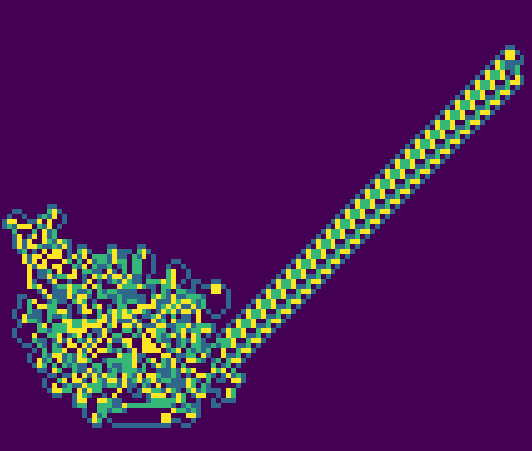
\includegraphics[width=0.2\textwidth]{reportTemplate/figures/lrlr_sin_base.png}
    \caption{Hormiga LRLR sin base tras 13,000 iteraciones.}
    \label{fig:lrlr_sin_base}
\end{figure}

\begin{figure}[h!]
    \centering
    
\includegraphics[width=0.2\textwidth]{reportTemplate/figures/lrlr_13000.png}
    \caption{Hormiga LRLR sobre base LLLR tras 3,000 iteraciones.}
    \label{fig:lrlr_13000}
\end{figure}





\subsection{Ejmplo:LRR sobre la base LLR}

En este ejemplo se compara el comportamiento de la hormiga con el patrón \textbf{LRR} en dos escenarios: sin una base predefinida y sobre una base configurada con el patrón \textbf{LLR}. La comparación permite observar cómo la infraestructura inicial afecta la estabilización y propagación de los patrones.

    \begin{figure}[h!]
        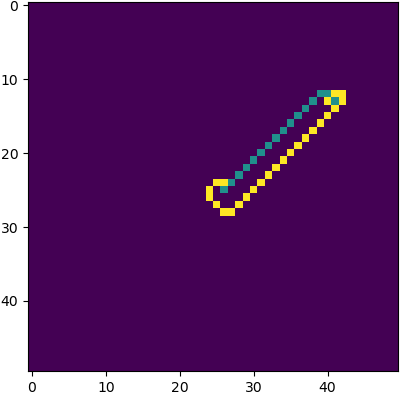
\includegraphics[width=0.2\textwidth]{reportTemplate/figures/llr.png}
        \caption{Configuración inicial de la base LLR tras 615 iteraciones.}
        \label{fig:llr_615}
    \end{figure}
    \hfill
    \begin{figure}[h!]
        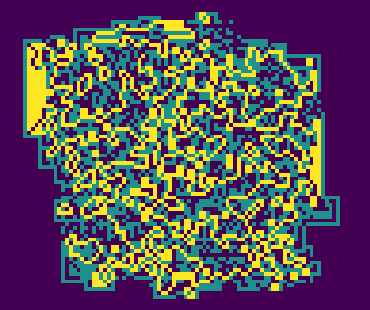
\includegraphics[width=0.2\textwidth]{reportTemplate/figures/lrr_sin_base.png}
        \caption{Hormiga LRR sin base tras 100,000 iteraciones.}
        \label{fig:lrr_no_base}
    \end{figure}
    \hfill
    \begin{figure}[h!]
        
\includegraphics[width=0.2\textwidth]{reportTemplate/figures/lrr_con_base.png}
        \caption{Hormiga LRR sobre base LLR tras 3,000 iteraciones.}
        \label{fig:lrr_base_llr}
    \end{figure}


En el primer escenario (Figura~\ref{fig:llr_615}), la base \textbf{LLR} genera un camino unidireccional y estable tras 615 iteraciones. Este camino lineal simplifica el espacio de la cuadrícula, proporcionando una infraestructura organizada que facilita la estabilización de patrones más complejos.

En el segundo escenario (Figura~\ref{fig:lrr_no_base}), la hormiga \textbf{LRR} opera sin una base predefinida. En este caso, su comportamiento es caótico, generando altos niveles de entropía y dispersándose sin formar un patrón claro incluso tras 100,000 iteraciones.

Por último, en el tercer escenario (Figura~\ref{fig:lrr_base_llr}), la hormiga \textbf{LRR} interactúa con la base \textbf{LLR}. Aquí, la estabilización ocurre rápidamente en solo 3,000 iteraciones, lo que demuestra cómo una infraestructura inicial organizada puede facilitar la convergencia hacia patrones estables. Este comportamiento es comparable al de un "virus artificial", que aprovecha la infraestructura preexistente para establecerse de manera eficiente y sostenida.
\section{Aumento de Escala: Activación de Múltiples Hormigas Virus}

En este experimento, exploramos cómo se comporta un sistema con cuatro hormigas virus interactuando secuencialmente. Cada hormiga activa opera directamente sobre el camino generado por las anteriores, lo que amplifica la complejidad del sistema y permite observar la interacción acumulativa.

\subsection{Descripción del Proceso}
El sistema comienza con la activación de la primera hormiga virus, que genera un patrón lineal estable sobre la base inicial. Este patrón sirve como infraestructura para la siguiente hormiga, que actúa directamente sobre el camino creado y lo amplía con su propio comportamiento. A medida que se activan las hormigas subsecuentes, cada una interactúa con el entorno acumulado, generando patrones cada vez más complejos.

\subsection{Resultados Observados}
Las figuras a continuación muestran los patrones generados por cada una de las hormigas virus en su activación:
\begin{itemize}
    \item \textbf{Hormiga Virus 1}: Genera un patrón lineal básico que sirve como base inicial (Figura~\ref{fig:virus1}).
    \item \textbf{Hormiga Virus 2}: Actúa sobre el camino de la Hormiga Virus 1, generando bifurcaciones en el patrón (Figura~\ref{fig:virus2}).
    \item \textbf{Hormiga Virus 3}: Amplifica las bifurcaciones y comienza a generar patrones caóticos y de alta entropía (Figura~\ref{fig:virus3}).
    \item \textbf{Hormiga Virus 4}: Combina los patrones acumulados en un entorno estructuralmente complejo con regiones organizadas y caóticas (Figura~\ref{fig:virus4}).
\end{itemize}

\subsection{Figuras de Activación}

\begin{figure}[h!]
    \centering
    
\includegraphics[width=0.45\textwidth]{virus1.png}
    \caption{Patrón generado por la Hormiga Virus 1.}
    \label{fig:virus1}
\end{figure}

\begin{figure}[h!]
    \centering
    
\includegraphics[width=0.45\textwidth]{virus2.png}
    \caption{Patrón generado por la Hormiga Virus 2 sobre el camino de la Hormiga Virus 1.}
    \label{fig:virus2}
\end{figure}

\begin{figure}[h!]
    \centering
    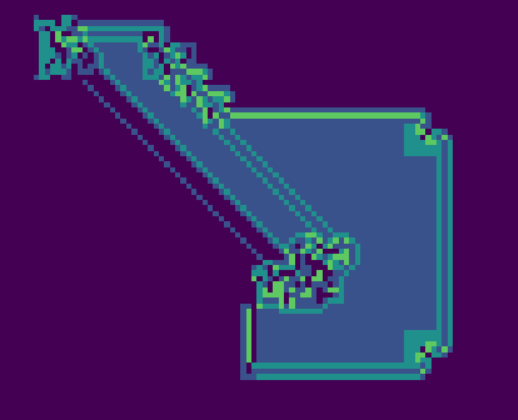
\includegraphics[width=0.45\textwidth]{virus3.png}
    \caption{Patrón generado por la Hormiga Virus 3 sobre los caminos acumulados.}
    \label{fig:virus3}
\end{figure}

\begin{figure}[h!]
    \centering
    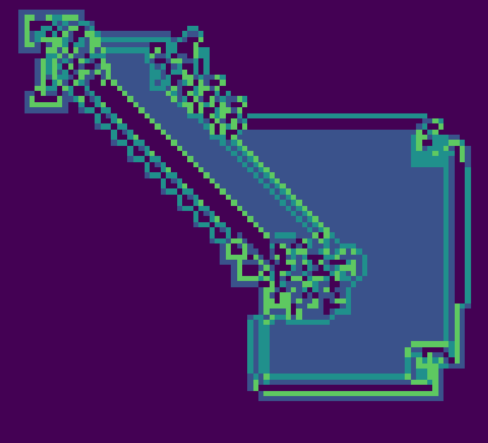
\includegraphics[width=0.45\textwidth]{virus4.png}
    \caption{Patrón generado por la Hormiga Virus 4, combinando los patrones acumulados.}
    \label{fig:virus4}
\end{figure}

\subsection{Análisis e Implicaciones}
Este experimento demuestra cómo un sistema estructurado puede amplificar la complejidad a través de interacciones acumulativas entre agentes. Cada hormiga actúa sobre el camino previo, lo que permite observar patrones emergentes y dinámicas virales que reflejan comportamientos de replicación y propagación.

En futuras investigaciones, sería interesante explorar cómo varían los patrones al modificar el tiempo de activación entre hormigas o cambiar las reglas del sistema base.                                                                                                                           

\section{Metodología y Configuración Experimental}

Para llevar a cabo este trabajo, utilizamos la supercomputadora \textit{Xiuhcoatl} del CINVESTAV, la cual permitió realizar cálculos intensivos mediante procesamiento paralelo. Diseñamos un experimento en el que cada procesador ejecutó una simulación de un posible virus, seleccionado de entre las hormigas que no se estabilizaron en experimentos previos con configuraciones de hasta 12 colores.

Escogimos la base configurada en el patrón RR...RL porque, tras un piloto inicial con varias configuraciones, esta resultó ser el mejor candidato. En la mayoría de los ejemplos del piloto se lograron observar comportamientos similares a los de un virus. Esto permitió utilizar esta configuración como un entorno estructurado que favorece la interacción con agentes virales.

Cada posible virus interactuaba con la hormiga base configurada en este patrón, cuya longitud de ADN variaba según el número de colores del virus. Las iteraciones de la hormiga base dependían del tamaño inicial de la matriz; para ello, consideramos matrices de tamaño entre 1000 y 1150, incrementando 10 unidades en cada caso. La hormiga base se detenía automáticamente al llegar a 4 celdas del borde de la matriz, generando un entorno estructurado sobre el cual los virus podían interactuar.

Las hormigas seleccionadas para actuar como virus fueron aquellas que no lograron estabilizarse en una iteración de hasta 100,000,000. En este experimento, diseñamos 16 programas que exploraron configuraciones de hormigas desde 3 hasta 9 colores, limitándonos a hormigas que comenzaban en la dirección R, ya que aquellas que iniciaban con L no producían resultados similares. Cada programa evaluó 32 hormigas, identificando las que no se estabilizaban; estas se ejecutaron sobre los 15 tamaños de hormiga base especificados, en simulaciones de hasta 10 millones de iteraciones. En total, se exploraron 4800 configuraciones posibles.

La supercomputadora \textit{Xiuhcoatl} proporcionó los recursos necesarios para este trabajo, utilizando 16 servidores con 32 procesadores cada uno y 64GB de RAM, lo que suma un total de 512 procesadores y 1024GB de RAM. Este trabajo se realizó durante una semana, con un tiempo de procesador total de 22991946,7764 segundos.



\section{Resultados Obtenidos}

Siguiendo nuestra definición de estabilización, logramos identificar un total de $1626$ virus y $540$ tiempos de estabilización distintos. La cantidad de virus detectados por cada color de ADN se detalla en el Cuadro \ref{tab:TB1}. Estos resultados sugieren una dependencia exponencial entre la cantidad de colores en el ADN y el número de virus, como se observa en la Figura \ref{fig:SLP}. Esta relación nos permite vislumbrar cómo un entorno estructurado puede amplificar comportamientos replicativos en estos agentes, logrando estabilizaciones aceleradas que imitan el comportamiento viral teorizado.

Los datos recopilados pueden consultarse en el siguiente enlace: 
\href{https://github.com/almuoz90/hormiga1/tree/e0f04899c7bebcd6a5a330093a3246662f58e2a8/Parasitos}{GitHub - Virus}

\begin{table}[h!]
\centering
\resizebox{8cm}{!} {
\begin{tabular}{rr|r|r}
  \hline
 & \textbf{Colors} & \textbf{Amount of virus (AV)} & \textbf{Log\_AV} \\ 
  \hline
& 0 & 0 &  \\ 
& 4 & 30 & 1.48 \\ 
& 5 & 60 & 1.78 \\ 
& 6 & 106 & 2.02 \\ 
& 7 & 217 & 2.34 \\ 
& 8 & 428 & 2.63 \\ 
& 9 & 785 & 2.89 \\ 
   \hline
\end{tabular}
}
 \caption{Cantidad de virus por cada color de ADN}
  \label{tab:TB1}
\end{table}

 \begin{figure}[h!]
        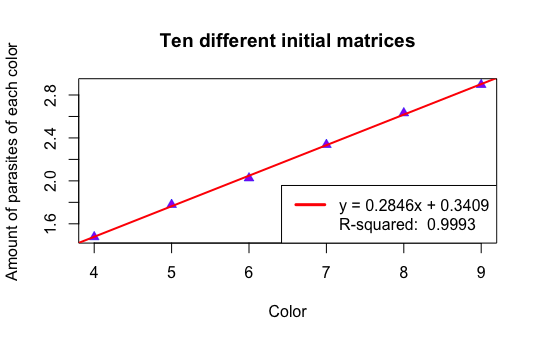
\includegraphics[width=0.5\textwidth]{reportTemplate/figures/SWPL.png}
  \caption{Relación entre el número de colores en el ADN y la cantidad de virus (Log\_AV).}
  \label{fig:SLP}
\end{figure}


\end{multicols}\end{document}